%& -job-name=Beck_Evaluation
\documentclass[10pt]{article}

% \usepackage{cite}

\usepackage{pythonhighlight}

%%%%% Text %%%%%
\usepackage[utf8]{inputenc} % Encode accents
% \usepackage[english]{babel}
\usepackage{textcomp} %supports the Text Companion fonts, which provide many text symbols (such as baht, bullet, copyright, musicalnote, onequarter, section, and yen), in the TS1 encoding.
\usepackage{xspace}
\usepackage[normalem]{ulem} % underlining that can stretch between words and be broken across lines

%%%%% Figures, tables and drawings %%%%%
\usepackage{pgfplots}
\usepackage{float} % For objects that won't fit into the page, such as figures and tables
\usepackage[footnotesize]{caption}
% \usepackage{subcaption}
\usepackage{subfig}
\usepackage{graphicx}
\usepackage{tabularx}
\usepackage{booktabs} % Nice tables
\usepackage{circuitikz}
\usetikzlibrary{external}
\tikzexternalize % activate!
\captionsetup[figure]{font=footnotesize,labelfont=footnotesize}
\captionsetup[table]{skip=1pt}

% \pgfplotsset{compat=newest}
% \pgfplotsset{plot coordinates/math parser=false}

%%%%% Maths %%%%
\usepackage{amsmath, amsbsy, amssymb, amsthm, amsfonts} 
\usepackage{mathtools} % for norm command, floor, veil...
\usepackage{mathrsfs}
\usepackage{multirow}
\usepackage{gensymb} % Provides \degree, \celsius, \perthousand, \micro and \ohm
\usepackage{cancel} % Cancel term in equation.
% \usepackage{empheq} % Boxed equations
% \usepackage{chemist}
% \usepackage[squaren,Gray]{SIunits}
% \usepackage{siunitx}

% Put black square at the end of proofs.
\renewcommand{\qedsymbol}{$\blacksquare$}
\newtheorem{theorem}{Theorem}[section]
\newtheorem{lemma}[theorem]{Lemma}
\newtheorem{proposition}[theorem]{Proposition}
\newtheorem{corollary}{Corollary}
\newtheorem{conjecture}{Conjecture}[section]
\theoremstyle{definition}
\newtheorem{definition}{Definition}[section]
\newtheorem{example}{Example}[section]
\newtheorem{remark}{Remark}
\newtheorem{assumption}{Assumption}

% % %%%%% Algorithms %%%%%
% % \usepackage{algorithmic}
% % \usepackage{algorithm}
% % \usepackage[ruled,vlined,linesnumbered,ruled,lined,boxed,commentsnumbered]{algorithm2e} 
% % \usepackage{comment}
% % \SetKwComment{Comment}{$\triangleright$\ }{}
% % \usepackage{sidecap}
% % \sidecaptionvpos{figure}{c}
% % %%% Code to be able to remove algorithm numbering
% % \makeatletter
% % \newcommand{\RemoveAlgoNumber}{\renewcommand{\fnum@algocf}{\AlCapSty{\AlCapFnt\algorithmcfname}}}
% % \newcommand{\RevertAlgoNumber}{\algocf@resetfnum}
% % \makeatother


%%%%% Appearance, font, ... %%%%%
%Margin size%
% \setlength{\headheight}{26pt}
% \addtolength{\oddsidemargin}{-.275in}
% \addtolength{\evensidemargin}{-.275in}
% \addtolength{\textwidth}{0.7in}
% \addtolength{\topmargin}{-.875in}   % White space from bottom
% \addtolength{\bottommargin}{-.875in}   % White space from bottom
% \addtolength{\textheight}{0.8in}
\footskip = 20pt
% \usepackage[top=2.cm,bottom=2.2cm,left=2cm,right=2cm]{geometry}
\usepackage[top=1.5cm,bottom=2.0cm,left=1.2cm,right=1.2cm]{geometry}
\usepackage{fancyhdr}
\usepackage{setspace}
\usepackage{lscape}
\usepackage{pdfpages} % Add other pdfs into.
\usepackage{xcolor}
\pgfplotsset{compat=newest}
\pgfplotsset{plot coordinates/math parser=false}
\newlength\figureheight
\newlength\figurewidth
\pgfplotsset{compat=newest}
\pgfplotsset{plot coordinates/math parser=false}

%%%%% Hypperlinks %%%%%
\usepackage[hyphens]{url}
\usepackage[hidelinks]{hyperref}
	
% %____________Newcommands__________________________________________________________
% \newcommand{\equaltext}[2]{\ensuremath{\stackrel{\text{#1}}{=}}}

%% Shorter commands
\newcommand{\bb}{\mathbb}
\newcommand{\bs}{\boldsymbol}
\newcommand{\cl}{\mathcal}
\newcommand{\ol}{\overline}
\newcommand{\fs}{\mathsf} % Sans serif
\newcommand{\wt}{\widetilde}
\newcommand{\wh}{\widehat}
\newcommand{\st}{%
  \ifmmode% math mode
  \mathrm{s.\!t.}%
  \else%
  s.\!t.\@\xspace%
  \fi%
}
\newcommand{\ie}{\emph{i.e.} }
\newcommand{\eg}{\emph{e.g.}, }
\newcommand{\etal}{\emph{et al.}}

% Ensembles and sets
\newcommand{\Rbb}{\bb{R}} % Real ensemble
\newcommand{\Cbb}{\bb{C}} % Complex ensemble
\newcommand{\Nbb}{\bb{N}} % Naturals ensemble
\newcommand{\Zbb}{\bb{Z}} % Integers ensemble

% Transformations
\newcommand{\tinv}[1]{{\textstyle\frac{1}{#1}}}
\newcommand{\inv}[1]{\frac{1}{#1}} % Inverse
\newcommand{\abs}[1]{\left\lvert#1\right\rvert} % absolute value
\newcommand{\sign}{{\rm sign}} % sign
\newcommand{\fft}[1]{\cl{F}\left\{#1\right\}} % Fourier transform
\newcommand{\fftt}[1]{\cl{F}_{2}\left\{#1\right\}} % 2D Fourier transform
\newcommand{\ifft}[1]{\cl{F}^{-1}\left\{#1\right\}} % Inverse Fourier transform
\newcommand{\ifftt}[1]{\cl{F}_{2}^{-1}\left\{#1\right\}} % Inverse Fourier transform

% Complex
\newcommand{\im}{\mathrm{i}\mkern1mu} % Complex number i
\newcommand{\real}[1]{\Re{\left\{#1\right\}}} % Real part
\newcommand{\imag}[1]{\Im{\left\{#1\right\}}} % Imaginary part
\newcommand{\conj}[1]{#1^{*}} % Conjuguate transpose

% Proba - Stats
\newcommand{\rv}{{\rm r.v.}\xspace}
\newcommand{\Prob}{{\bb{P}}}
\newcommand{\proba}[1]{\bb{P}\left[#1\right]}
\newcommand{\pdf}{\varphi}
\DeclareMathOperator{\Var}{Var}
\DeclareMathOperator{\Cov}{Cov}
% \newcommand{\E}[1]{\bb{E}\left[#1\right]} % Expectation
\newcommand{\E}[2][]{\bb{E}_{#1}\left[#2\right]} % Expectation
\newcommand{\expec}[1]{\mathop{{}\mathbb{E}}_{#1}} % for mathematical expectation
\newcommand{\distiid}{\sim_{\iid}} % iid distributed
\newcommand{\iid}{%
  \ifmmode% math mode
  \mathrm{i.i.d.}%
  \else%
  i.i.d.\@\xspace%
  \fi%
}

% Others
\newcommand{\limit}[2]{\underset{#1 \rightarrow #2}{\text{lim}}} % limit
\newcommand{\ud}{\mathrm{d}} % Infinitesimal part for integration
\newcommand{\supp}{{\rm supp}\,} % Support
\DeclareMathOperator{\tr}{tr} % Trace
\DeclareMathOperator{\diag}{diag}
\newcommand{\transpose}[1]{#1^\top} % Transpose
\newcommand{\modulo}[2]{{/#1/}_{#2}} % Modulo
\newcommand{\norm}[2]{\left\lVert#1\right\rVert_{#2}} % p-norm
% \DeclarePairedDelimiterX{\norm}[1]{\lVert}{\rVert}{#1} % Norm of something,
\newcommand{\scp}[3][]{#1\langle #2, #3 #1\rangle} % Scalar product
\newcommand{\fro}[2]{\langle #1, #2 \rangle_{\text{F}}} % Frobenius inner product
\DeclareMathOperator*{\argmax}{arg\,max}
\DeclareMathOperator*{\argmin}{arg\,min}
\DeclareMathOperator{\prox}{prox}
\DeclareMathOperator{\proj}{proj}
\DeclareMathOperator{\Id}{\mathds{1}}
\DeclareMathOperator{\dom}{dom}
\DeclareMathOperator{\diam}{diam}
\newcommand{\lpn}[3]{\ell_{#1,#2}^{#3}}

% Commands specific to evaluation
\newcommand{\soft}[1]{\cl T_{#1}}
\newcommand{\ATA}{\bs A^\top \bs A}

% %___________________________________________________________________________________

\makeatletter
\newcommand{\mathleft}{\@fleqntrue\@mathmargin0pt}
\newcommand{\mathcenter}{\@fleqnfalse}
% Defines a new command for the horizontal lines, change thickness here
\newcommand{\HRule}{\rule{\linewidth}{0.5mm}} 

%%%%%%%%%%%%%%%%%%%%%% Headers and footers %%%%%%%%%%%%%%%%%%%%%%%%%%
\fancypagestyle{firstpage}{%
    % \chead{\includegraphics[width=1\textwidth]{Telsiks2021-header.pdf}}
    \lfoot{978-1-6654-4442-2/21/\$31.00~\copyright2021 IEEE} 
    \renewcommand{\headrulewidth}{0pt}
    \cfoot{\thepage}
}

\fancypagestyle{others}{%
    \cfoot{\thepage}
    \renewcommand{\headrulewidth}{0pt}
}

\hoffset = 0cm % Decalage gauche-droite
\voffset = 0.0cm % Decalage haut-bas
%%%%%%%%%%%%%%%%%%%%%%%%%%%%%%%%%%%%%%%%%%%%%%%%%%%%%%%%%
    
%%%%%%%%%%%%%%% Make references colors %%%%%%%%%%%%%%%%%%
\usepackage{hyperref}
\hypersetup{
    colorlinks=true,
    linkcolor=black,
    filecolor=magenta,      
    urlcolor=cyan,
    citecolor = magenta
}
\usepackage{cleveref}
\crefformat{equation}{(#2\color{blue}#1#3)} 
%%%%%%%%%%%%%%%%%%%%%%%%%%%%%%%%%%%%%%%%%%%%%%%%%%%%%%%%

%% Comments
\newcommand{\LJc}[1]{\textcolor{blue}{\textbf{\scriptsize [LJ: #1]}}}
\newcommand{\OLc}[1]{\textcolor{orange}{\textbf{\scriptsize [OL: #1]}}}
\newcommand{\TODO}[1]{\textcolor{red}{\textbf{\scriptsize [TODO: #1]}}}
\newcommand{\edt}[1]{{\color{blue} #1}}
\newcommand{\del}[1]{{\color{red} \sout{#1}}}

\newcommand{\br}[1]{\textcolor{red}{[\textbf{BR:#1}]}}
\renewcommand{\br}[1]{}
\newcommand{\rev}[1]{{ #1}}
%\newcommand{\rev}[1]{{\color{blue} #1}}

%%%%%%%%%%%%%%%%%%%%%%%%%%%%%%%%%%%%%%%%%%%%%%%%%%%%%%%%%%
%%%%%%%%%%%%%%%%%%%%%%%%%%%%%%%%%%%%%%%%%%%%%%%%%%%%%%%%%%


%% SPECIFIC COMMANDS

\begin{document}

\begin{center} % Center everything on the page
 
%----------------------------------------------------------------------------------------
%	HEADING SECTIONS
%----------------------------------------------------------------------------------------

\HRule \\[0.2cm]
{ \huge \bfseries First-order methods in optimization - Evaluation }\\[0.1cm] % Title of your document
\HRule \\[0.4cm]
 
Olivier Leblanc, Guillaume Thiran. \\

%----------------------------------------------------------------------------------------
%	DATE SECTION
%----------------------------------------------------------------------------------------

% \vfill % Fill the rest of the page with whitespace
% \

% {\large \today ~~~~~~~~~~~~~~~~~~~~~~~~~~~~~~~~~~~~~~~~~~~~~~~Academic year 2019-2020}\\[1cm] % Date, change the \today to a set date if you want to be precise
\end{center}

%%%%%%%%%%%%%%%%%%%%%%%%%%%%%%%%%%%%%%%%%%%%%%%%%%%%%%%%%%%%%%%%%%%%%

%%%%%%%%%%%%%%%%%%%%%%%%%%%%%%%%%%%%%%%%%%
\section{Part 1 - Slide 45}
%%%%%%%%%%%%%%%%%%%%%%%%%%%%%%%%%%%%%%%%%%
%
%%%%%
\subsection{6. (with code)}
%
\begin{equation*}
    f(\bs x) = 2 x_{[1]} + x_{[2]} 
    = \max_{\bs y} \left\{ \sum_{i} y_i x_i; \sum_i y_i=3, 0 \le
    y_i \le 2 \right\} = \sigma_{\{ \bs y|\bs 1^\top \bs y = 3, 
    \bs 0 \le \bs y \le 2 \bs 1 \}}.
\end{equation*}
%
Hence,
%
\begin{equation*}
    \prox_f(\bs x) = \bs x - \cl P_{\{ \bs y|\bs 1^\top \bs y = 3, 
    \bs 0 \le \bs y \le 2 \bs 1 \}} (\bs x).
\end{equation*}
%
Writing $C=\{ \bs y|\bs 1^\top \bs y = 3, 
\bs 0 \le \bs y \le 2 \bs 1 \}$, it can be compared with 
$H_{\bs a, b} \bigcap \text{Box}[\bs l, \bs u]$, with 
$\bs a=\bs 1, b=3, \bs l=\bs 0, \bs u = \bs 2$.
%
\begin{python}
import numpy as np
def error_fct(a,b,l,u,x,mu):
    y = projbox(x-mu*a,l,u)
    return error = a@y-b
     
def projbox(x, l, u):
    return np.minimum(np.maximum(x,l), u)

def proj_H_inter_box(a,b,l,u,x):
    mu_low = -1 #start with guesses for mu-levels
    mu_high = 1
    #check that the levels give respectively negative and positive values
    #for the function error = a@y-1 with y = proj_box(l,u,x-mu*a)
    #positive for lower bound
    j=0
    j_max =100
    error_l = -1
    while (error_l<0) & (j<j_max) :
        mu_low = mu_low*2 #more negative
        error_l=error_fct(a,b,l,u,x,mu_low)
        j=j+1
    #negative for upper bound
    k=0
    k_max =10
    error_h = 1
    while (error_h>0) & (k<k_max) :
        mu_high = mu_high*2 #more positive 
        error_h=error_fct(a,b,l,u,x,mu_high)
        k=k+1

    i = 0
    i_max = 100
    tol = 1e-8
    error = 2*tol
    while (np.abs(error)>tol) & (i<i_max) :
        mu_mid = (mu_low+mu_high)/2
        error = error_fct(a,b,l,u,x,mu_mid)
        if error>0:
            mu_low = mu_mid
        else:
            mu_high = mu_mid
        i=i+1

    #Compute the solution with the good level
    return projbox(x-mu_mid*a,l,u)

def proxf(x):
    return x - proj_H_inter_box(np.ones(len(x)),3,np.zeros(len(x)),2*np.ones(len(x)),x)

x = np.array([2,1,4,1,2,1])
print(proxf(x))
\end{python}
%
The output is : $[1.5, 1., 2.,  1.,  1.5, 1. ]$.
%
%%%%
\subsection{8.}
%
\begin{equation*}
    f(t) = \left\{
        \begin{array}{ll}
          1/t,~~t>0, \\
            \infty,~~ \text{else}.
        \end{array}
      \right.
\end{equation*}
%
\begin{equation*}
    \prox_{\lambda f}(t) = \argmin_u \left\{
        \begin{array}{ll}
            \lambda/{ u},~~u>0, \\
            \infty,~~ \text{else}.
        \end{array}
    \right. + \tinv 2 \norm{u-t}{2}^2 
\end{equation*}
%
Clearly, the minimum occurs when $u>0$, i.e. on the differentiable part. Hence,
%
\begin{equation*}
    \frac{-\lambda}{u^2} + u - t = 0 \Leftrightarrow 
    u^3 - tu^2-\lambda=0,
\end{equation*}
and it can be checked the second derivative is always positive on $u>0$, implying it exists a unique solution of the above and it corresponds to a minimum. Finally,
%
\begin{equation}
    \prox_{\lambda f}(t) = \{ u>0 | u^3 
    - tu^2-\lambda=0  \}.
\end{equation}
%
%%%%
\subsection{9.}
%
\begin{equation*}
    f(\bs X) = \left\{
        \begin{array}{ll}
          \tr \bs X^{-1},~~\bs X \succ 0, \\
            \infty,~~ \text{else}.
        \end{array}
    \right.
    = \left\{
        \begin{array}{ll}
        \sum_{i=1}^n \tinv{\lambda_i},~~\bs X \succ 0, \\
            \infty,~~ \text{else}.
        \end{array}
    \right. 
\end{equation*}
%
As one can write $f(\bs X) = g(\lambda_1(\bs X), \cdots,
\lambda_n(\bs X)) = \sum_{i=1}^n h(\lambda_i)$, $f$ is a \emph{symmetric spectral function}.
%
With the EigenValue Decomposition (EVD) of $\bs X$ as 
$\bs X = \bs U \diag{\lambda (\bs X)} \bs U^T$, this gives
%
\begin{align*}
\begin{split}
    \prox_{\lambda f} (\bs X) &= \bs U \diag(\prox_{\lambda g} 
    [\lambda_1,\cdots, \lambda_n]) \bs U^\top \\
    &= \bs U \diag(\prox_{\lambda h} (\lambda_1), \cdots,
    \prox_{\lambda h} (\lambda_n)) \bs U^\top \\
    &= \bs U \diag(\{\{ u>0| u^3-\lambda_i u^2-\lambda=0 \}\}_{i=1}^n)
    \bs U^\top,
\end{split}
\end{align*}
with $h(t)=\frac{1}{t}$ for $t>0$. 
%
%%%%%
\subsection{10.}
%
\begin{equation*}
    \lambda f(\bs x) = \lambda (\norm{\bs x}{2}-1)^2 
    = \lambda \norm{\bs x}{2}^2
    - 2 \lambda \norm{\bs x}{2} + \lambda.
\end{equation*}
%
Using the provided tables, one identifies it with 
$g(\bs x) + \frac{c}{2} \norm{\bs x}{2}^2 + \scp{\bs a}{\bs x}
+ \gamma$, with $g(\bs x) = -2\lambda\norm{\bs x}{2}, c=2\lambda,
\bs a=\bs 0, \gamma=0$.
Hence,
%
\begin{equation*}
    \prox_{\lambda f}(\bs x) = 
    \prox_{\frac{-2\lambda\norm{\cdot}{2}}{1+2\lambda}}
    \bigg(\frac{\bs x}{1+2\lambda} \bigg) = 
    \left\{
        \begin{array}{ll}
            \left( 1+ \frac{2\lambda}{\norm{\bs x}{2}} 
            \right) \frac{\bs x}{1+2\lambda},~~\bs x \neq \bs 0, \\
            \{ \bs u: \norm{\bs u}{}= \frac{2\lambda}{1+2\lambda} \},~~ \bs x = \bs 0.
        \end{array}
      \right.
\end{equation*}

%%%%%%%%%%%%%%%%%%%%%%%%%%%%%%%%%%%%%%%%%%
\section{Part 2 - Exercise 0 - slide 40}
%%%%%%%%%%%%%%%%%%%%%%%%%%%%%%%%%%%%%%%%%%
%
\begin{equation*}
    \min_{\bs x \in \Rbb^n}~\tinv 2 \norm{\bs{Ax}-\bs b}{2}^2
    + \underbrace{\frac{\lambda_1}{2} \norm{\bs x}{2}^2 
    + \lambda_2 \norm{\bs x}{1}}_{\text{elastic net}},
\end{equation*}
%
where $\bs A \in \Rbb^{m\times n}$, $\bs b \in \Rbb^m$ and 
$\lambda_1, \lambda_2>0$.
%
Choosing $f(\bs x) = \tinv 2 \norm{\bs{Ax}-\bs b}{2}^2 
+ \frac{\lambda_1}{2} \norm{\bs x}{2}^2$ as the $\sigma$-strongly 
convex and differentiable part and 
$g(\bs x) = \lambda_2 \norm{\bs x}{1}$ as the closed 
convex but non differentiable part, one has 
$\nabla f(\bs x) = \bs A^\top (\bs{Ax}-\bs b) + \lambda_1 
\bs{x}$ and $\prox_{\alpha g}(\bs x) = 
\soft{\alpha\lambda_2}(\bs x)$.
%
\begin{itemize}
    \item (\emph{Proximal Gradient})
    \begin{align*}
    \begin{split}
        \bs x^{k+1} &= \prox_{\tinv L g}(\bs x^k - \tinv L 
        \nabla f(\bs x^k)) \\
        &= \soft{\frac{\lambda_2}{L}} \left( \bs x^k 
        - \tinv L (\ATA + \lambda_1 \bs I) 
        \bs x^k + \tinv L \bs A^\top\bs b
        \right),
    \end{split}
    \end{align*}
    %
    with $L = \norm{\ATA + \lambda_1 \bs I}{}
    = \lambda_{\max} (\ATA) + \lambda_1 = \norm{\bs A}{2}^2
    + \lambda_1$.
    \item (\emph{FISTA})
    \begin{align*}
    \begin{split}
    \left\{
    \begin{array}{lll}
        \bs x^{k+1} &= \soft{\frac{\lambda_2}{L}} 
        \left( \bs y^k - \tinv L (\ATA + \lambda_1 \bs I) 
        \bs y^k + \tinv L \bs A^\top\bs b \right) \\
        t_{k+1} &= \frac{1+\sqrt{1+4t_k^2}}{2} \\
        \bs y^{k+1} &= \bs x^{k+1} + \left( 
        \frac{t_k-1}{t_{k+1}} \right) (\bs x^{k+1}- \bs x^k)
    \end{array}
    \right.
    \end{split}
    \end{align*}
    \item (\emph{V-FISTA})
    \begin{align*}
    \begin{split}
    \left\{
    \begin{array}{ll}
        \bs x^{k+1} &= \soft{\frac{\lambda_2}{L}} 
        \left( \bs y^k - \tinv L (\ATA + \lambda_1 \bs I) 
        \bs y^k + \tinv L \bs A^\top\bs b \right) \\
        \bs y^{k+1} &= \bs x^{k+1} + \left( 
        \frac{\sqrt\kappa-1}{\sqrt\kappa+1} \right) 
        (\bs x^{k+1}- \bs x^k),
    \end{array}
    \right.
    \end{split}
    \end{align*}
    %
    with $\kappa=L/\sigma$, and $\sigma=\lambda_{\min} (\bs A^\top \bs A)
    + \lambda_1 = \lambda_1$ if $\bs A$ is not full rank.
\end{itemize}
%
Now, if one chooses $f(\bs x) = \tinv 2 \norm{\bs{Ax}-\bs b}{2}^2$ 
as the differentiable (but not strongly convex) part and 
$\alpha g(\bs x) = \frac{\alpha\lambda_1}{2} \norm{\bs x}{2}^2 
+ \alpha\lambda_2 \norm{\bs x}{1}$ as the closed 
convex but non differentiable part, one has 
$\nabla f(\bs x) = \bs A^\top (\bs{Ax}-\bs b)$ and, 
by identification with $g'(\bs x) + \frac{c}{2} 
\norm{\bs x}{2}^2 + \scp{\bs a}{\bs x} + \gamma$ with 
$g'(\bs x) = \alpha\lambda_2 \norm{\bs x}{1}, 
c=\alpha\lambda_1, \bs a=\bs 0, \gamma=0$, 
$\prox_{\alpha g}(\bs x) = 
\prox_{\frac{\alpha}{\alpha\lambda_1+1} \lambda_2 
\norm{\cdot}{1}} (\frac{\bs x}{\alpha\lambda_1+1}) = 
\soft{\frac{\alpha\lambda_2}{\alpha\lambda_1+1}} 
(\frac{\bs x}{\alpha\lambda_1+1})$.
%
\begin{itemize}
    \item (\emph{V-FISTA2})
    \begin{align*}
    \begin{split}
        \left\{
        \begin{array}{ll}
            \bs x^{k+1} &= \soft{\frac{\lambda_2/L_2}{
            \lambda_1/L_2 + 1}} 
            \left( \frac{\bs y^k - \tinv{L_2} \bs A^\top  (\bs A
            \bs y^k-\bs b) }{\frac{\lambda_1}{L_2}+1} \right)
            = \soft{\frac{\lambda_2}{
                \lambda_1 + L_2}} 
                \left( \frac{L_2\bs y^k - \bs A^\top  (\bs A
                \bs y^k-\bs b) }{\lambda_1+L_2} \right) \\
            \bs y^{k+1} &= \bs x^{k+1} + \left( 
            \frac{\sqrt{\kappa_2}-1}{\sqrt{\kappa_2}+1} 
            \right) (\bs x^{k+1}- \bs x^k),
        \end{array}
        \right.
    \end{split}
    \end{align*}
    %
    with $L_2=\norm{\bs A}{2}^2$, $\kappa_2=L_2/\sigma$, 
    and $\sigma=\lambda_1$ (given by the statement).
\end{itemize}

\begin{figure}[H]
    \centering
    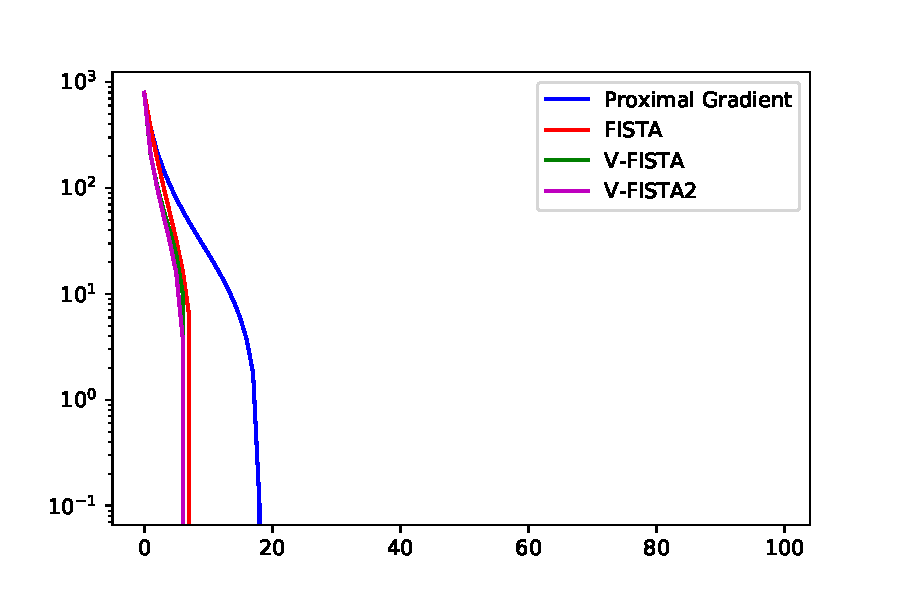
\includegraphics[width=14cm]{images/part2_ex0.pdf}
    \caption{$F(\bs x^k)-F_{\text{opt}}$ in log-scale along the 
  y-axis for the first 100 iterations of each of the methods 
  with all-zeros vectors and a constant stepsize. }
  \label{fig: ex0}
\end{figure}
%
As can be observed in Fig.~\ref{fig: ex0}, the V-FISTA 
methods worked the best, with a slight improvement in 
V-FISTA which does not follow the theory.
The four first elements are:
\begin{itemize}
    \item (-0.43969331  0.01974521  1.42280231 -0.87819581)
    \item (-0.4319773   0.02881602  1.43373682 -0.9066518 )
    \item (-0.43210834  0.0295975   1.43437285 -0.90583213 )
    \item (-0.43210892  0.02959727  1.43437048 -0.9058291 )
\end{itemize}
%
for the four methods, PG, FISTA,
V-FISTA, V-FISTA2, respectively.
%%%%%%%%%%%%%%%%%%%%%%%%%%%%%%%%%%%%%%%%%%
\section{Part 2 - Exercise 1 - slide 41}
%%%%%%%%%%%%%%%%%%%%%%%%%%%%%%%%%%%%%%%%%%
%
\begin{equation*}
    \min_{\bs x \in \Rbb^{30}} \sqrt{\bs x^\top \bs{Qx} + 
    2 \bs b^\top \bs x + c} + 0.2 \norm{\bs{Dx+\bs 1}}{1},
\end{equation*}
%
where $\bs Q \in \Rbb^{30\times 30}$, $\bs b\in \Rbb^{30}$, $c\in \Rbb$, $\bs D
\in \Rbb^{30\times 30}$. The matrix $\bs Q$ is positive definite. \\

\indent (a) The first step of the problem is to show it is well-defined (i.e. $\bs x^\top \bs{Qx} + 
2 \bs b^\top \bs x + c\geq 0$ if $c> \bs b^\top\bs Q^{-1} \bs b$.). To that aim, letting the Cholesky factorisation of $\bs Q$ being denoted as $\bs Q = \bs L^\top \bs L$, 
\begin{align*}
	\bs x^\top \bs{Qx} + 
2 \bs b^\top \bs x + c &= \bs x^\top \bs{Qx} + \bs b^\top \bs L^{-1} \bs{Lx} + \bs x^\top \bs L^\top \bs L^{-\top} \bs b + \bs b^{\top} \bs L^{-1} \bs L^{-\top} \bs b - \bs b^\top \bs L^\top \bs L^{-\top} \bs b + c,\\
&= \left \| \bs{Lx} + \bs L^{-\top} \bs b \right \|_2^2 + c -\bs b^\top\bs Q^{-1} \bs b. 
\end{align*}  
From the above, as a norm is always nonnegative, one can conclude the problem is well-defined if $c> \bs b^\top\bs Q^{-1} \bs b$.   \\
%
\indent (b) Starting from the norm expression, one can obtain 
\begin{align*}
	\sqrt{\bs x^\top \bs{Qx} + 
    2 \bs b^\top \bs x + c} + 0.2 \norm{\bs{Dx+\bs 1}}{1} &= \left \| \begin{matrix}
    \bs{Lx} + \bs L^{-\top} \bs b \\
    \sqrt{c -\bs b^\top\bs Q^{-1} \bs b}
    \end{matrix} \right \|_2 + 0.2 \norm{\bs{Dx+\bs 1}}{1}. 
\end{align*}
As a norm is convex, as a composition with a  linear mapping preserves convexity and since a sum of convex functions is convex, the problem is convex. \\
\indent (c) To fit the framework of FISTA,  we denote by $f(\bs x) = \sqrt{\bs x^\top \bs{Qx} + 
2 \bs b^\top \bs x + c}$ and $g(\bs x) =  0.2 \norm{\bs{Dx+\bs 1}}{1}$ where $g$ is proper, closed and convex, and $f$ is $L_f$-smooth and convex. More precisely, the Lipschitz constant of $f$ can be identify by computing its Hessian: 
\begin{align*}
\bs \nabla f(\bs x) & = \frac{\bs{Qx}+\bs b}{\sqrt{\bs x^\top \bs{Qx} + 
2 \bs b^\top \bs x + c}}, \\
\bs \nabla^2 f(\bs x) & = \frac{\bs Q}{\sqrt{\bs x^\top \bs{Qx} + 
2 \bs b^\top \bs x + c}} - \frac{(\bs{Qx}+\bs b)(\bs{Qx}+\bs b)^\top}{\left(\bs x^\top \bs{Qx} + 
2 \bs b^\top \bs x + c\right)^{\frac{3}{2}}}. 
\end{align*}
The latter can be bounded as 
\begin{align*}
	\bs \nabla^2 f(\bs x) \preceq  \frac{\bs Q }{\sqrt{\bs x^\top \bs{Qx} + 
2 \bs b^\top \bs x + c}} = \frac{\bs Q }{ \sqrt{c -\bs b^\top\bs Q^{-1} \bs b} \sqrt{1+\frac{\left \| \bs{Lx} + \bs L^{-\top} \bs b \right \|_2^2}{ c -\bs b^\top\bs Q^{-1} \bs b}}} \preceq \frac{\bs Q }{ \sqrt{c -\bs b^\top\bs Q^{-1} \bs b}},
\end{align*}
leading to $L_f = \frac{\lambda_{\text{max}}\left(\bs Q\right)}{\sqrt{c -\bs b^\top\bs Q^{-1} \bs b}}$. In the case of the exercise, we obtain $L_f = 53.54$ and thus a step size of  $0.019$. \\
As $\bs D \bs D^\top = \bs I$, one can compute the proximal operator of $\alpha g$ as 
\begin{align*}
	\prox_{\alpha g}(\bs x) & = \bs x + \bs D^\top \left( 
\soft{0.2\alpha} (\bs{Dx}+\bs 1) - \bs{Dx} - \bs 1 \right),\\
 & =  \bs D^\top 
\soft{0.2\alpha} (\bs{Dx}+\bs 1) -\bs D^\top \bs 1 .
\end{align*}
This leads to 
\begin{itemize}
    \item (\emph{Proximal gradient}):
    \begin{align*}
    \begin{split}
        \bs x^{k+1} &= \prox_{\tinv{L_f}g} (\bs x^k - \tinv{L_f} \nabla f(\bs x^k)) \\ 
        &=  \bs D^\top 
       \soft{\frac{0.2}{L_f}} \left[ \bs D(\bs x^k - \tinv{L_f} \nabla 
        f(\bs x^k) ) + \bs 1 \right]  - \bs D^\top  \bs 1    \\
        &= \bs D^\top  \soft{\frac{0.2}{L_f}} \left[ 
        \bs D(\bs x^k - \tinv{L_f} \frac{\bs{Qx}^k+\bs b}{\sqrt{(\bs x^k)^\top 
        \bs{Qx}^k + 2 \bs b^\top \bs x^k + c}} ) + \bs 1 \right] - \bs D^\top \bs 1 .
    \end{split}
    \end{align*}
    
    \item (\emph{FISTA}):
      \begin{align*}
    \begin{split}
    \left\{
    \begin{array}{lll}
        \bs x^{k+1} &= \bs D^\top  \soft{\frac{0.2}{L_f}} \left[ 
        \bs D(\bs y^k - \tinv{L_f} \frac{\bs{Qy}^k+\bs b}{\sqrt{(\bs y^k)^\top 
        \bs{Qy}^k + 2 \bs b^\top \bs y^k + c}} ) + \bs 1 \right] - \bs D^\top \bs 1 \\
        t_{k+1} &= \frac{1+\sqrt{1+4t_k^2}}{2} \\
        \bs y^{k+1} &= \bs x^{k+1} + \left( 
        \frac{t_k-1}{t_{k+1}} \right) (\bs x^{k+1}- \bs x^k)
    \end{array}
    \right.
    \end{split}
    \end{align*}
\end{itemize}
\begin{figure}[H]
    \centering
    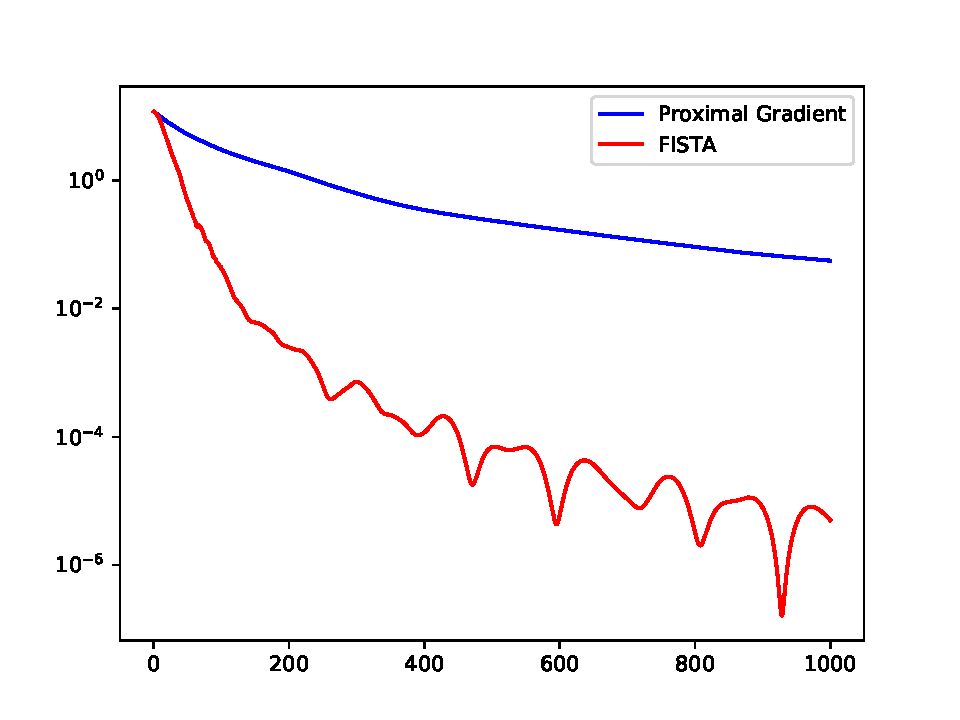
\includegraphics[width=14cm]{images/part2_ex1.pdf}
    \caption{$F(\bs x^k)-F_{\text{opt}}$ in log-scale along the 
  y-axis for the first 1001 iterations of each of the methods 
  with all-zeros vectors and a constant stepsize. The optimal solution has been computed as the best one across 10000 iterations.  }
  \label{fig: ex0}
\end{figure}
       Vector found by PG: 
       \begin{align*}
       \bs x^{*,\text{PG}} &= [0.406, -0.093, -0.093, -0.874, -1.025, -0.044,  0.521, -1.16 ,
        0.877,  0.129, -0.242,  1.664,  1.32 , -0.561, -0.079, -1.764,\\& \qquad 
       -1.351, -0.387, -1.158,  0.844,  0.43 , -0.715, -0.349, -0.037,
        1.408, -0.971,  1.206,  0.795,  0.568,  1.284].
       \end{align*}
       Vector found by FISTA: 
\begin{align*}\bs x^{*,\text{FISTA}} &= [-0.455, -0.389,  0.291, -1.149, -1.309, -0.43 ,  0.667, -1.434,
        1.082, -0.019, -0.416,  1.732,  1.293, -0.541, -0.143,\\& \qquad  -1.704,
       -1.396, -0.742, -1.539,  0.335, -0.218, -0.662, -0.151, -0.085,
        1.801, -0.566,  1.321,  0.849,  0.701,  1.091].\end{align*}

%
%%%%%%%%%%%%%%%%%%%%%%%%%%%%%%%%%%%%%%%%%%
\section{Part 2 - Exercise 3 - slides 71-72}
%%%%%%%%%%%%%%%%%%%%%%%%%%%%%%%%%%%%%%%%%%
%
Given a set of data points $\bs x_1, \bs x_2,\cdots,\bs x_n \in \Rbb^d$ and 
corresponding labels $y_1,y_2,\cdots,y_n$. The soft margin SVM problem is given 
by 
\begin{equation*}
    \min \left\{\tinv 2\norm{\bs w}{2}^2+C \sum_{i=1}^{n} \max 
    \left\{0,1-y_i \bs w^\top \bs x_i\right\}\right\}
\end{equation*}
%
\indent (a) \\
%
\\
\indent (b) \\





\end{document}
